% THIS IS A LATEX TEMPLATE FILE FOR PAPERS INCLUDED IN THE
% *Anthology of Computers and the Humanities*. ADD THE OPTION
% 'final' WHEN CREATING THE FINAL VERSION OF THE PAPER. 
% DO NOT change the documentclass
\documentclass[final]{anthology-ch} % for the final version
%\documentclass{anthology-ch}         % for the submission

% LOAD LaTeX PACKAGES
\usepackage{booktabs}
\usepackage{graphicx}
% ADD your own packages using \usepackage{}

% TITLE OF THE SUBMISSION
% Change this to the name of your submission
\title{Unstable Data and the Unusual Case of the Prosody Excerpt in the Digital Library}

% AUTHOR AND AFFILIATION INFORMATION
% For each author, include a new call to the \author command, with
% the numbers in brackets indicating the associated affiliations 
% (next section) and ORCID-ID for each author.  
\author[1]{Rebecca Sutton Koeser}[
  orcid=0000-0002-8762-8057
]

\author[1]{Mary Naydan}[
  orcid=0000-0002-7960-3175
]

% While we encourage including ORCID-IDs for all authors, you can
% include authors that do not have one by definining an empty ID.
%\author[1,2]{Meredith Martin}[
\author[1]{Meredith Martin}[
  orcid=0000-0003-0214-8757
]

% There should be one call to \affiliation for each affiliation of
% the authors. Multiple affiliations can be given to each author
% and an affiliation can be given to multiple authors. 
\affiliation{1}{Center for Digital Humanities, Princeton University, Princeton, New Jersey, USA}
%\affiliation{2}{English Department, Princeton University, Princeton, New Jersey, USA}

% KEYWORDS
% Provide one or more keywords or key phrases seperated by commas
% using the following command
\keywords{humanities data, unstable data, reproducibility, digital libraries}

% METADATA FOR THE PUBLICATION
% This will be filled in when the document is published; the values can
% be kept as their defaults when the file is submitted
\pubyear{2025}
\pubvolume{1}
\pagestart{1}
\pageend{1}
\conferencename{Proceedings of Conference XXX}
\conferenceeditors{Editor1 Editor2}
\doi{00000/00000}  

\addbibresource{bibliography.bib}

%%%%%%%%%%%%%%%%%%%%%%%%%%%%%%%%%%%%%%%%%%%%%%%%%%%%%%%%%%%%%%%%%%%%%%%%%%%
% HERE IS THE START OF THE TEXT
\begin{document}

%TC:ignore
\maketitle 


\begin{abstract}
Stable data is essential for repeatable research, and cultural heritage data is an invaluable resource for computational humanities research, but the fluctuations within this kind of data pose challenges to reproducible, repeatable, and follow-up research. This paper uses the case study of HathiTrust Digital Library content within the Princeton Prosody Archive (PPA), particularly excerpted and augmented content, as a window into the surprising instability of this large-scale data. We analyze the rate of change in PPA excerpted content, all of PPA, and all of HathiTrust resulting from HathiTrust updates. We use this case study to illuminate the degree of change in HathiTrust, as one exemplar of a cultural heritage data aggregator, which we think is not well understood by computational researchers, and to consider the implications for research.
\end{abstract}

\renewcommand{\thefootnote}{\fnsymbol{footnote}}
\footnote{Code and data for this paper is available at \href{https://github.com/rlskoeser/chr2025-unstable-data-paper/}{https://github.com/rlskoeser/chr2025-unstable-data-paper/} }
\renewcommand{\thefootnote}{\arabic{footnote}}
\setcounter{footnote}{0}

%TC:endignore

\section{Introduction}

Data is essential for computational humanities research. Whether research is based on small-scale data to test a particular method, expansive collections for measuring larger trends across time, or something in between, stable data is crucial to interpreting results. The ability to share or recreate a dataset is equally crucial for reproducible research and to assess, critique, and take up new methodologies. However, the ability to build on previous research is difficult when there is instability in research data sources, particularly when that instability is unexpected or incompletely understood. 

Stable data is particularly essential when it is used in novel or creative ways not anticipated by data publishers. Rufus Pollock, an early proponent of open knowledge and open data, has long argued that ``the best thing to do with your data will be thought of by someone else'' \cite{pollock_open_2011}. Computational humanists’ reliance on cultural heritage data poses particular challenges, since GLAM (Galleries, Libraries, Archives, and Museums) sector workflows and goals are not always aligned with computational research. In this paper, we share insights gained from our discovery of surprisingly unstable data in the integrated and enhanced content from the HathiTrust Digital Library within the Princeton Prosody Archive (PPA). This case study provides an opportunity to reflect on the gaps in current standards for reproducible research,  humanities and cultural heritage data publication, and computational humanities. 

In 2016, the FAIR Principles were published with the ``ultimate goal ... to optimise the reuse of data'' \autocite{noauthor_fair_nodate}. These guidelines include unique, persistent identifiers so data can be found, and documenting and structuring data according to community standards to support replication and combination.  In 2017, the first statement on ``Collections as Data'' was published, with a goal to  ``encourage computational use of digitized and born digital collections'' \autocite{noauthor_santa_nodate}. Reusable data is an important step towards many of the modes of work that Christof Schoch elaborates within the conceptual space of ``repetitive research'' \autocite{schoch_repetitive_2023}, but reusable data may not be sufficient. And data drawn from digital collections with greater ``changeability and instability'' require more detailed documentation on provenance and processing for reuse \autocite{burrows_reproducibility_2023}.  Many of the 2023 Collections as Data position statements offer glimpses of instability: items are accessioned, deaccessioned, and reappraised following curatorial workflows \autocite{knazook_building_2023}; there is ``considerable fluctuation'' in adding and updating resources \autocite{neudecker_collections_2023}; digital content should be treated as original, unique publications for preservation \autocite{steven_no_2023, roke_moving_2023}, and yet these developments reflect the ``destabilization of prior frameworks, theories, and practices'' \autocite{bailey_collections_2023}. The FAIR principles do not mention data versioning, and provide no guidance on granularity of identifiers, but our experience indicates both are necessary.

\section{Unstable data in the Princeton Prosody Archive}

\subsection{Princeton Prosody Archive }

The Princeton Prosody Archive (PPA) is an open-source, full-text searchable database of 6,000+ English-language digitized works about the study of poetry, versification and pronunciation \cite{noauthor_princeton_nodate}. The works in the PPA — which include grammar books, elocution manuals, and scholarly articles, among many other kinds of books — were all published between 1532 and 1928, the current cut-off year for works in the public domain in the United States.

The PPA initially integrated only full volumes from HathiTrust, but was designed for expansion to other sources. It is one of the only digital humanities resources to present full-text OCR, page image thumbnails, and bibliographic metadata from multiple databases in a single dynamic interface.\footnote{The PPA now also includes content from Gale/Cengage’s Eighteenth Century Collections Online (ECCO) and Early English Books Online using editions from the Text Creation Partnership (EEBO-TCP).} The PPA also now supports excerpted works, such as book chapters or journal articles, to focus the collection only on relevant portions of larger works.

\subsection{HathiTrust Digital Library}

The majority of the works in the PPA come from HathiTrust Digital Library, a US-based, not-for-profit consortium of over 60 academic and research libraries from across North America and other countries. HathiTrust Digital Library began in 2008 with Google’s mass digitization initiative and now provides ``reading access'' to its 18+ million digitized volumes ``to the fullest extent allowable by U.S. and international copyright law'' \cite{noauthor_welcome_nodate}.

Similar large-scale aggregators, often led by national libraries, exist in Europe and beyond. \textbf{TROVE}, maintained by the National Library of Australia, collects billions of digital items from Australian libraries, universities, museums, galleries, and archives \cite{noauthor_home_nodate}. \textbf{Gallica}, the digital library of the Bibliothèque nationale de France (BnF) and over 300 partners, provides access to over 10 million items \cite{noauthor_page_nodate}. \textbf{Europeana} makes available various kinds of media and accompanying metadata from thousands of cultural institutions \cite{noauthor_discover_nodate}. Smaller cultural heritage aggregators include Switzerland’s \textbf{e-rara} \cite{noauthor_e-rara_nodate} and \textbf{e-manuscripta} \cite{noauthor_e-manuscripta_nodate} and Finland’s \textbf{Finna} \cite{noauthor_search_nodate}. We mention these aggregators to suggest that the kinds of data instability we encountered in HathiTrust will be found in \textit{any }large-scale cultural heritage aggregator because of GLAM workflows to manage and improve collections, as well as the ephemeral nature of technical infrastructure. These changes often involve a trade-off between reproducibility and improvement. For example, TROVE’s crowdsourced text-correcting feature improves OCR transcripts, but means that researchers will be working with different transcripts depending on the date of download \cite{noauthor_text_nodate}. This opportunity for continued content enhancement is valuable, but depending on the extent of the changes, could have downstream effects on word-level analysis. As another familiar example, Europeana's metadata coordinators explain to their users why they might find broken links and how some of these can never be fixed \cite{noauthor_keeping_nodate}.

HathiTrust has a long history of enthusiastic collaboration with researchers and computational humanists. Many projects focused on methods for, first, finding certain material within HathiTrust’s massive digital library, and then testing text and data mining methods on that collection using the tools and services provided by HathiTrust Research Center (HTRC) \cite{noauthor_hathitrust_nodate}. Prominent examples of this two-step process include Gioia Stevens's \textbf{Early American Cookbooks} project (now a permanent collection within HathiTrust) \cite{stevens_new_2017} and Laure Thompson and David Mimno's \textbf{20th Century English-Language Speculative Fiction }(a recommended workset within HTRC) \cite{thompson_building_nodate, 
noauthor_recommended_nodate}. Recent work from Ryan Dubnicek and collaborators has focused on using machine learning methods to discover particular genres within HathiTrust Digital Library \cite{parulian_uncovering_2022, dubnicek_ryan_piloting_2023} and building out the customizable capacities of HTRC’s Extracted Features dataset through the development of an open API \autocite{walsh_library_2023}. The content is limited to HathiTrust items, and the algorithms, datasets, and advanced computing environments are all contained within HTRC’s platform.\footnote{In October 2024, HathiTrust announced that it will be shutting down HTRC because “many of our members have rarely utilized HTRC’s services,” leaving the future of TDM on HathiTrust works uncertain \cite{noauthor_plans_nodate}. }  

\subsection{PPA’s unusual use of HathiTrust}

Unlike most other projects, the PPA pulls content dynamically from multiple HathiTrust systems and combines it with content from non-HathiTrust sources, cutting across the boundaries of digital resources and adding a layer of technical complexity.\footnote{It is difficult to identify other digital projects with unusual uses of data or technical infrastructure; this requires insider knowledge of the processes and sources used to build projects, which is less often narrated than research methods, analytical results, or final outputs. Meredith Martin’s new monograph, \textit{Poetry’s Data}, is a notable exception to this trend and argues for the value of narrating the process of navigating our digital research infrastructures \cite{martin_poetrys_2025}. The Princeton Geniza Project and the Shakespeare \& Company Project are two additional examples of unexpected use: both projects attach research data to digital images published by GLAM institutions via International Image Interoperability Framework (IIIF) APIs \cite{noauthor_princeton_nodate, noauthor_shakespeare_2020}. This kind of persistent use is within the guidelines of the published IIIF APIs, but atypical.}  PPA uses HathiTrust’s API to import bibliographic metadata, which it presents alongside page-level data (OCR) from local copies of METS XML and plain text files accessed via rsync and page image thumbnails dynamically loaded from HathiTrust’s image server.

In addition, the PPA enhances the data pulled from HathiTrust, particularly for excerpts. Whereas HathiTrust indexes full works and journal volumes, the PPA enables searching and browsing at the more granular level of the book chapter or journal article. The bibliographic metadata for prosody-related excerpts had to be identified and curated manually \cite{naydan_book_2024}, providing a level of specificity not available in HathiTrust.

While HathiTrust was an enthusiastic partner and participated in several rounds of negotiations about how PPA would access their data, it eventually become clear — especially through the case of the prosody excerpt — that their infrastructure was not designed to be used by external projects in this persistent, dynamic manner. 

\subsubsection{The problem of excerpts}

The instability of HathiTrust's data was first evidenced when excerpt-level functionality was added to the PPA. Suddenly, there were mismatches between the thumbnail images and full-text snippets. Page ranges were incorrect. How was this possible? We realized that because the PPA was regularly pulling content from multiple HathiTrust systems at different intervals, HathiTrust's routine rescanning of its material could alter the digital page numeration that was used to specify excerpt ranges.

We suspect that HathiTrust's regular rescanning is not widely known or even fully understood among researchers. The main public indication is the following disclaimer on an ``About'' page (emphasis added): ``\textit{The HathiTrust collection is not static.} Works get added to the collection every day, and \textit{sometimes a digital item may be updated with a new version}. Bibliographic records can be updated when contributors send us corrections. Copyright and access statuses may change as items undergo copyright review or we receive permissions agreements from copyright holders'' \cite{noauthor_how_nodate}. 

To address this problem, we sought a solution to automate fixing range changes whenever HathiTrust made updates. At first glance, this task seemed computationally tractable. Figure  \ref{fig:code-comparison} shows the page-level metadata for the same set of pages on two different dates and the types of changes that occur. Some of the changes involve recharacterizing page-level semantic metadata (e.g. flagging \texttt{UNTYPICAL\_PAGE} or renumbering section starts), though it is worth noting that the updated attributes are not always more accurate. For PPA excerpts, we were most interested in the relative changes between the \texttt{seq} field (digital page index) and the \texttt{pageNum} field (page number in the source edition).

%TC:ignore
\begin{figure}
    \centering
    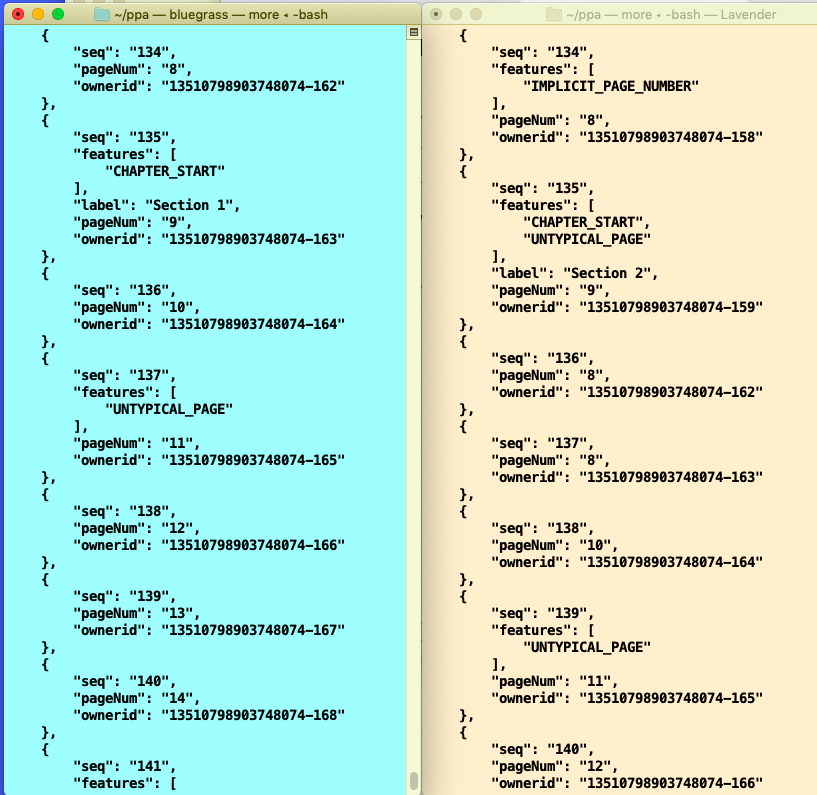
\includegraphics[width=0.5\linewidth]{figures/y.png}
    \caption{Side-by-side screenshots showing page-level metadata for ``The Scansion of Middle English Alliterative Verse'' by William E. Leonard \cite{noauthor_scansion_nodate}, generated from the page's HTML and JavaScript, on two different dates: March 18, 2024 (left) and March 26, 2024 (right). Note the change in \texttt{pageNum} beginning at \texttt{seq} 136.}
    \label{fig:code-comparison}
\end{figure}
%TC:endignore

Digging deeper, we discovered complex edge cases in page numeration that would make automation difficult, if not impossible, such as articles with \textit{three} different page numbers for a single page (see Figure \ref{fig:MLN}).

%TC:ignore
\begin{figure}
    \centering
    \includegraphics[width=1\linewidth]{figures/Screenshot 2025-07-10 at 3.19.38 PM.png}
    \caption{The above page from O. F. Emerson’s ``The Development of Blank Verse: A Study of Surrey'' in the journal \textit{Modern Language Notes} \cite{emerson_o_f_development_1889} displays three different page numbers. Each column of \textit{MLN }gets its own page number (left, 467; right, 468), and each page gets a third, found at the bottom center (234). HathiTrust's black navigation controls show that it takes the upper left page number as the original/physical page number (p. 467). This convention is not the most intuitive, and it means that scrolling through HathiTrust's reader, the original page numbers increase by two instead of one. The digital page number/sequence number (\#296) is based on scanning and subject to change with rescanning.}
    \label{fig:MLN}
\end{figure}
%TC:endignore

After the technical cost of automatically fixing page ranges became apparent, the PPA team resolved that manual correction was the best solution.

\section{Quantifying HathiTrust's rate of change}

\subsection{Changes in PPA excerpts}

A November 2023 spreadsheet used by the PPA team to correct excerpt page ranges provides a window into the degree of instability. After we discovered that the PPA was pulling erroneous content for some excerpts, we tasked a student researcher with manually checking and correcting the page ranges. We discovered that out of 517 total excerpts, 121 (23.4\%) had changed over the course of two years. For 10 of those, the length of the excerpt changed, in most cases by two pages.\footnote{There were two outliers with differences in length of 25 and 16 pages; preliminary investigations suggest that these were due to data errors in the original excerpts. For instance, one excerpt was originally only pulling a single page when the article was actually several pages long; most likely, someone neglected to input the end range. However, it is difficult to confirm with certainty after the fact.} This might occur if, for instance, a digital edition included a duplicated page, which was later found and removed. Excerpt starting pages shifted an average of 6.4 pages; 9 volumes shifted by more than 10 pages, and one extreme outlier, Thomas Stewart Omond's ``Swinburne as a Metrician'' in volume 76 (1909) of \textit{The Academy and literature} \cite{omond_thomas_stewart_swinburne_1909}, shifted by 240 pages! This could happen if HathiTrust replaced a partial scan with a more complete one. Most troubling, when we analyze the overlap between pages in range before and after these updates, there are 36 excerpts with \textit{no pages in common} between the initial and updated page range; that is, without updating the page range, we would be including \textit{none} of the intended contents. While small shifts in page numeration are negligible for a massive collection like HathiTrust, for smaller, curated, scholar-focused projects, even small changes like these can have big implications, leading to errors in scholarship, confusion among users, and distrust in the quality of the resource.

\subsection{Changes in all of HathiTrust}

Observing this volatility at the small scale of PPA excerpts led us to wonder about the rate of change for PPA content more generally and in HathiTrust at scale. Fortunately for us, HathiTrust is incredibly transparent about changes to its collection — at least at a high level. In addition to emails HathiTrust regularly sends out with lists of records that are no longer public domain, which dataset users must remove from their copy of HathiTrust data (see Appendix \ref{appdx:ht-dataset-dist} and \ref{appdx:ht-deletion-email}), HathiTrust publishes monthly and daily files with data about updated records. They note that a volume might be included in this update file for \textit{any} of the following reasons: it was newly deposited, an existing item was replaced with a new copy, there were changes to rights and access permissions, or the bibliographic metadata was updated \cite{noauthor_hathifiles_nodate}. While the occurrence of an update is therefore relatively easy to track, identifying the exact \textit{type} of change is not so easy.\footnote{Our investigations made it clear that the modification time of the METS XML file corresponds to the date in the public version label on the full view page for individual items. The text content could be modified before or after this time. } Figure \ref{fig:hathi-daily-updates} charts the number of updated volumes across all of HathiTrust from May 1 to July 10, 2025.
\begin{figure}[t!]
    \centering
    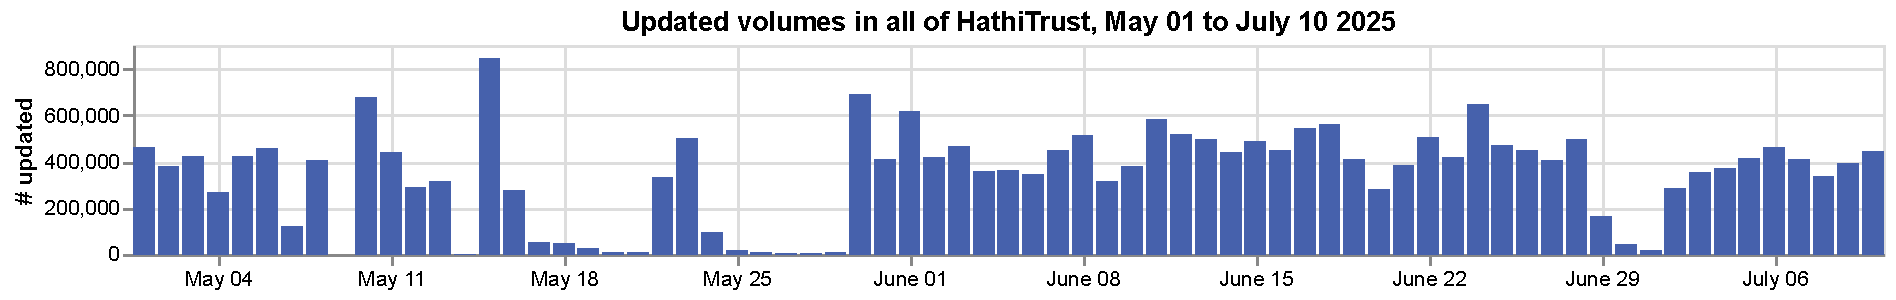
\includegraphics[width=1\linewidth]{figures/hathitrust_changes_countonly.pdf}
    \caption{Number of volumes updated daily in all of HathiTrust from May 1 to July 10, 2025.}
    \label{fig:hathi-daily-updates}
\end{figure}
The number of updates varies on any given day from nearly negligible to more than 800,000 volumes. The day with the most updates during this time period was May 15, 2025 with 846,329 volumes updated (4.5\% of all of HathiTrust). The average daily update over this period is 348,392, which is only 1.8\% of all of HathiTrust.

\subsection{Changes in all of PPA}

What about all the HathiTrust volumes within the Princeton Prosody Archive? How frequently are they changing? One way to answer this question is to filter the data on HathiTrust updates to volumes included in PPA; when we do, we find that PPA updates track somewhat with the larger updates (refer to Figure \ref{fig:ppa-daily-updates} and compare with Figure \ref{fig:hathi-daily-updates}). Although these changes are on a much smaller scale, there are still multiple days when more than a hundred volumes changed.

\begin{figure}[t!]
    \centering
    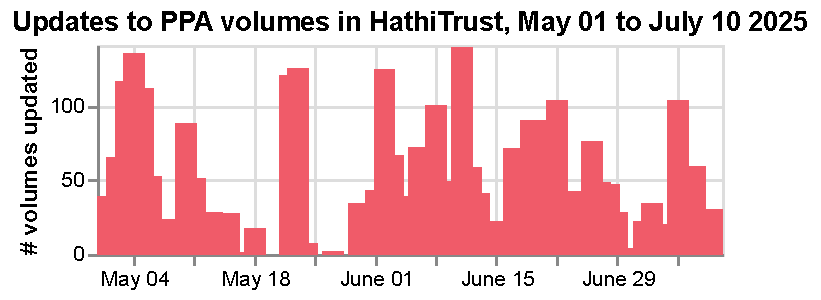
\includegraphics[width=1\linewidth]{figures/ppa_hathitrust_changes_countonly.pdf}
    \caption{Number of PPA HathiTrust volumes updated daily from May 1 to July 10, 2025.}
    \label{fig:ppa-daily-updates}
\end{figure}

Another way to investigate this question is by comparing two different snapshots of the PPA full-text corpus. We created one version that was last updated November 2024 and another in February 2025, a difference of roughly three months.\footnote{The earlier version is the corpus that has been used as the basis for computational research on PPA; the later one was generated as part of a matching text and image snapshot which was provided as a one-time dataset by HathiTrust.} There are slight differences between the number of pages in these two versions, with a little over 1.5 million pages in common. When we match pages based on exactly equal text contents within the same volume (excluding pages with no text), we find 855,930 (55.8\%) matching pages across the two corpora; of those, 14,423 pages (1.7\% of the total 1.5 million pages) have shifted sequence within their volume, indicating a change in structure with no update to the text. The mismatches for the remaining pages (44.2\% of our corpus) are likely due to OCR changes. While it is appealing to think that the content has been improved, this means that any word or token-level analysis on the prior version of the corpus would need to be either rerun or realigned to the updated text.\footnote{The PPA's ECCO data provides an interesting counterpoint to the instability of HathiTrust: the data itself is unchanged, and the OCR text for these materials have not been updated since 2008, in spite of the known poor quality of the text and substantial improvements in OCR technology since the collection was originally digitized \cite{hill_quantifying_2019}.}

\subsection{Implications}

The difficulty of dealing with HathiTrust's frequent changes factored into the PPA team's decision to shift from maintaining a dynamic database to extracting the data and making the full-text corpus useful for computational analysis instead. One project aimed to detect and identify lines of poetry quoted across the million+ pages in the PPA. Systematically identifying these poems was a first step towards answering research questions about English prosody; a dataset of poem excerpts could illuminate when and how particular poets or poems became the exemplars for poetic forms or figures of speech, or how quickly after publication a poet’s work becomes a canonical example, or the network of examples being reused from other prosodists.

As we considered approaches to poetry detection within PPA, one collaborator suggested levering  Ted Underwood's dataset of page-level genre predictions for HathiTrust volumes \cite{underwood_page-level_2014}. This dataset includes such granular predictions because, as the researchers note, volumes are rarely a single genre and often collect disparate materials. While the genre prediction task is not equivalent to poetry detection, there is some overlap in goals. Pages labeled as poetry could be used as a starting point or confirmation of results from other methods, an approach which would fall under reuse of data or follow-up research, in Schoch's terminology \autocite{schoch_repetitive_2023}. However, the degree of change possible in HathiTrust materials means that this page-level data is basically unusable. As a demonstration of this problem, we offer one example: the essay ``On Stile and Versification'' by William Belsham \cite{belsham_stile_1799} appears in Underwood's dataset and in the PPA. Figure \ref{fig:poetry_pages} shows the only two pages in the essay that are majority poetry and discusses the discrepancies in page sequence numbers between the two datasets. Figure \ref{fig:poetry_exc_pages} shows the very brief poetry excerpts that occur in the rest of the essay and discusses how they are characterized.

%TC:ignore
\begin{figure}[hbt!]
  \centering
  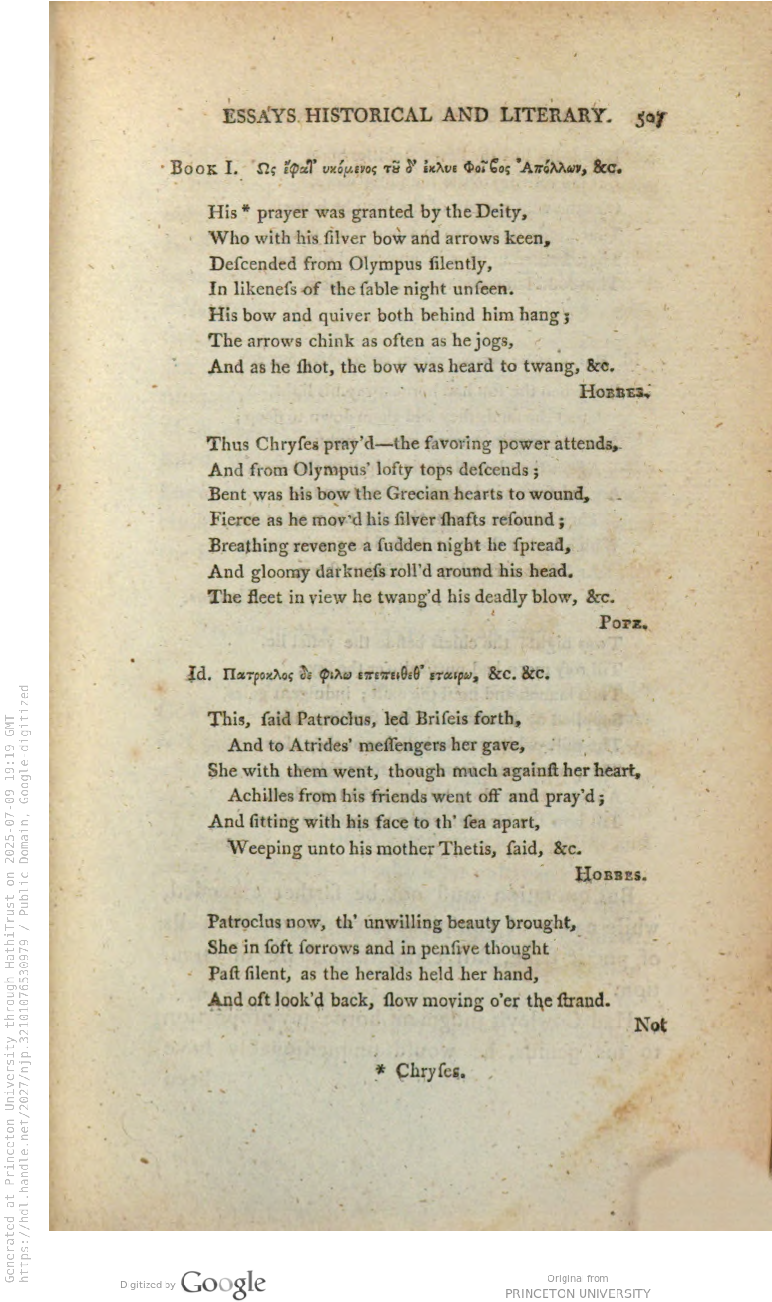
\includegraphics[width=0.35\linewidth]{figures/hathi-pages/njp-32101076530979-515-1752088772.pdf}
  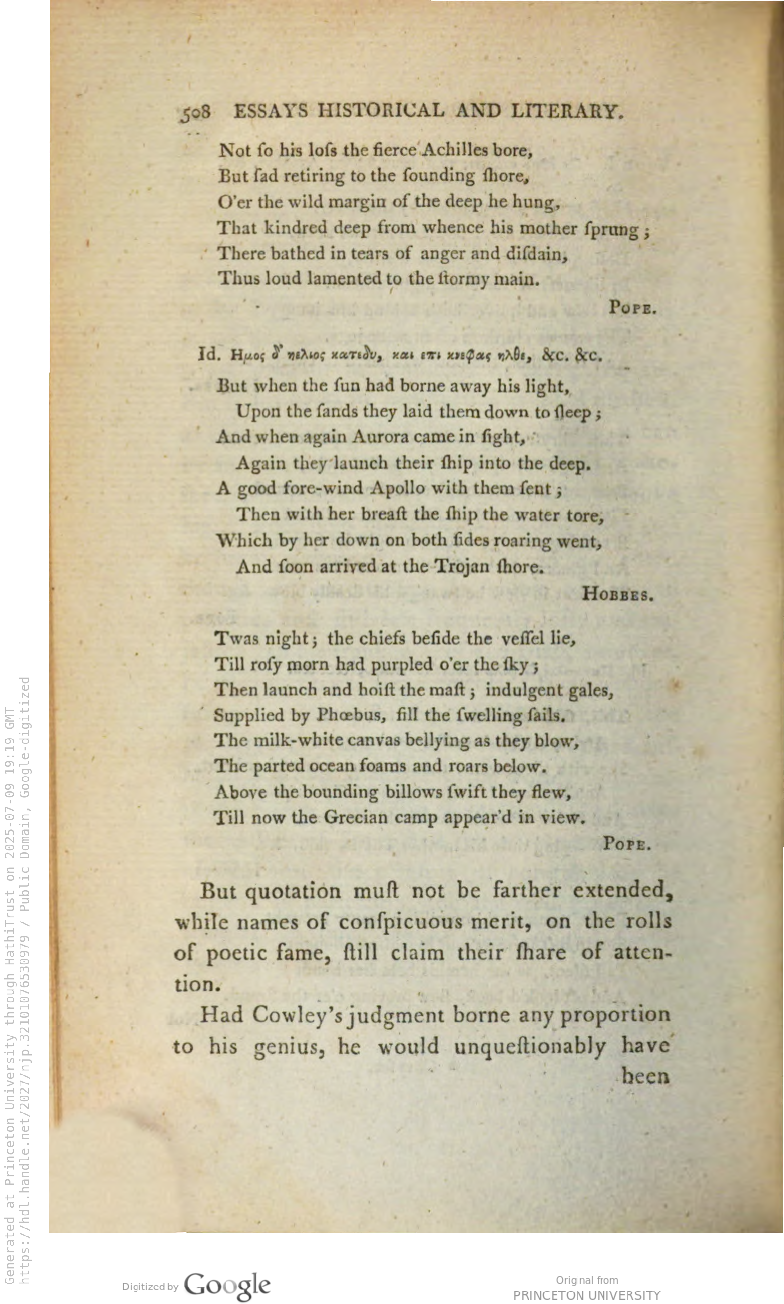
\includegraphics[width=0.35\linewidth]{figures/hathi-pages/njp-32101076530979-516-1752088741.pdf}
  \caption{The only two pages in this essay that are majority poetry. Underwood's dataset could potentially help us find poem excerpts like these. However, in the PPA's updated dataset, the digital sequence numbers for these two pages are 515 and 516. In Underwood's page-level genre metadata, the only two pages labeled ``poetry'' are digital pages 510 and 511. Images courtesy of HathiTrust.}
  \label{fig:poetry_pages}
\end{figure}

\begin{figure}[hbt!]
  \centering
  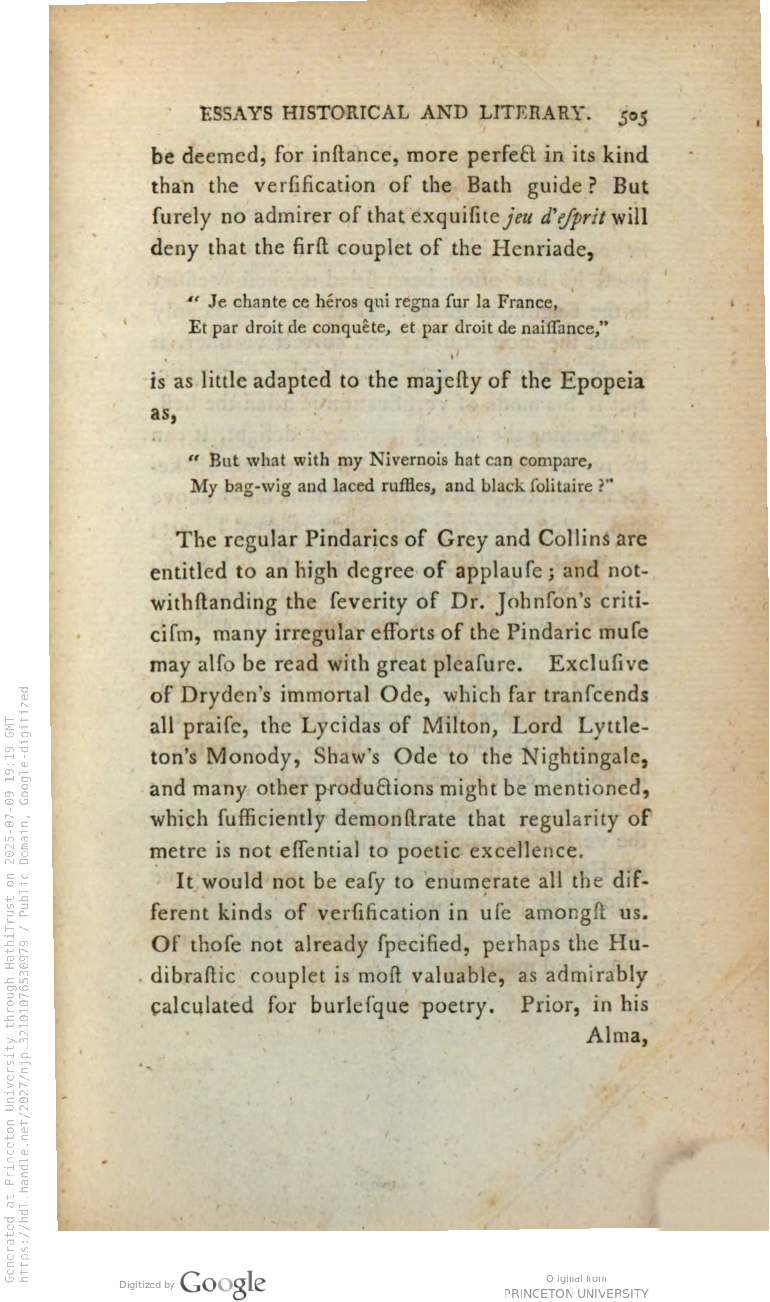
\includegraphics[width=0.35\linewidth]{figures/hathi-pages/njp-32101076530979-513-1752088792.pdf}
  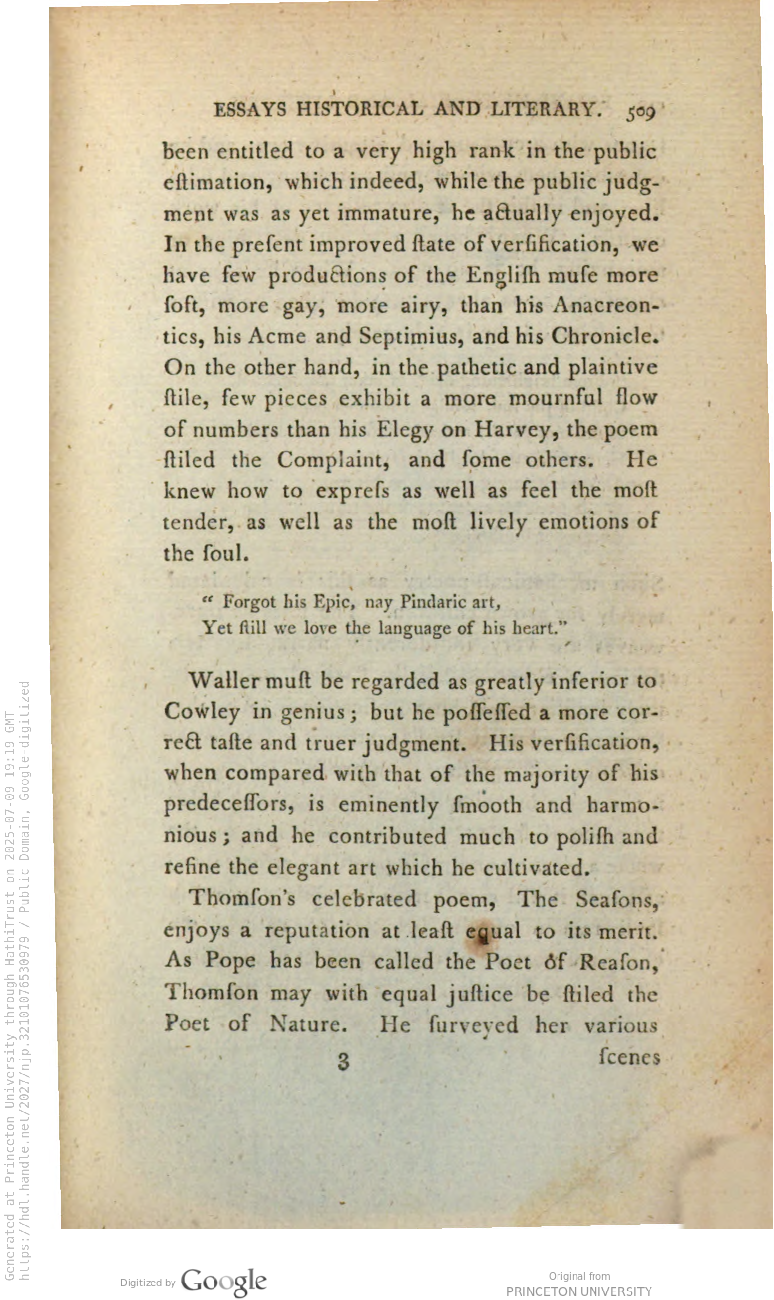
\includegraphics[width=0.35\linewidth]{figures/hathi-pages/njp-32101076530979-517-1752088752.pdf}
  \caption{Two pages with short poetry excerpts. In Underwood's dataset, pages like these are classified as ``nonfiction prose'' rather than poetry. Underwood's dataset would therefore not help us find short poetry excerpts like these. Images courtesy of HathiTrust.} 
  \label{fig:poetry_exc_pages}
\end{figure}
%TC:endignore

This example shows that page-level genre predictions have potential for research questions within PPA or other projects based on HathiTrust materials, but updates in HathiTrust content make them unusable for work on different versions of the data.

Like Underwood, the PPA project team is using digital sequence to refer to pages in the found-poems dataset. What do we do with the fact that this dataset, like Underwood's, refers to a snapshot of HathiTrust and the PPA at a moment in time? For researchers working with HathiTrust data, there is no stable page identifier across time. A stable page ID for HathiTrust is not feasible due to the scale of labor involved in creating and maintaining HathiTrust, since there are so many individual libraries with their own workflows feeding into the aggregator. While this lack of stable referents is therefore understandable, it nevertheless poses a problem for computational research and reproducibility that the field has yet to solve. 

\section{Conclusions}

There are many different methods and approaches for computational research on large-scale corpora and digital collections. Because of the complexity of reconciling augmented, curated PPA data with ongoing HathiTrust updates, we have followed the familiar pattern of working with a frozen snapshot of a corpus to test our methods and generate a new derivative dataset, which will be the basis for additional research. It is important to have research results linked to a specific version of a dataset, which can be cited and potentially shared, depending on permissions. However, this approach has downsides; even within our own project, our desires to refine the dataset and enhance the metadata run the risk of introducing unintentional changes into the corpus and becoming out of sync with work derived from the previous version. These challenges are even more substantial beyond the bounds of an individual project, making it difficult to share research results for reuse, critical review, follow-up research, or to feed back into enhancing and augmenting critical heritage datasets and digital collections. 

Ideally, cultural heritage data and computational research constitute a virtuous cycle: data is used to test new methods or algorithms and to make domain-specific arguments, and results feed back into improvements to data, methods, and new scholarly arguments through repeated and follow-up research. GLAM institutions and researchers are often related but not perfectly aligned in their goals, and researchers may often require different scales, nuance, and complexity than can be supported by curatorial workflows. A crucial first step is to be transparent about the degree and scope of instability in data, and to publish and use versioned data whenever feasible. FAIR does not go far enough, and we must develop new community standards, whether for versioning or more granular identifiers, as well as tools or methods to work more robustly with unstable data for reproducible, repeatable research.  

%TC:ignore
\section*{Acknowledgements}

...

% Print the biblography at the end. Keep this line after the main text of your paper, and before an appendix. 
\printbibliography

% You can include an appendix using the following command 

\pagebreak
\appendix

\section{HathiTrust Statement for Dataset Distribution} \label{appdx:ht-dataset-dist}

By my signature, I acknowledge and confirm the following:

\begin{enumerate}
    \item  I am receiving texts from the University of Michigan that are made available under an agreement between my sponsoring institution - [indicate sponsoring institution, e.g., Dartmouth College] - and Google.
    \item  I have read this agreement and agree to abide by its terms and to use the texts in accordance with the statement of my research, as submitted to the University of Michigan.
    \item  I agree to notify the University of Michigan of any changes that are made in the scope or nature of my research.
    \item  I understand that volumes I receive from the University of Michigan may be determined at a later date to be in copyright. I agree to delete these volumes and any copies that have been made upon notification from the University of Michigan. I agree to notify the University of Michigan at feedback@issues.hathitrust.org to confirm deletion of any such volumes.
\end{enumerate}

\rule{\textwidth}{0.5pt}

Name \hspace{0.3\textwidth} Signature \hspace{0.3\textwidth} Date

\rule{\textwidth}{0.5pt}

Title

\rule{\textwidth}{0.5pt}

Email \hspace{0.3\textwidth}  Phone

\pagebreak 

\section{Example HathiTrust deletion email for public domain dataset} \label{appdx:ht-deletion-email}

\begin{verbatim}
Subject: Delete notifications for ht_text_pd dataset
From: HathiTrust <support@hathitrust.org>

Dear HathiTrust dataset recipient,

This email is to notify you that volumes in the HathiTrust
"ht_text_pd" dataset, of which you have downloaded all
or a subset of files, no longer meet the criteria for
inclusion in the dataset, and you no longer are allowed to
use them in your research.

Please review the data you have synced from HathiTrust to
check whether you have the volumes listed below. If so,
delete all copies you retain of these volumes in
accordance with our terms of use. Alternatively, you may
delete your copy of the dataset and re-sync to the updated
dataset.

If you no longer possess HathiTrust datasets, or if you
have other questions regarding datasets, then please email
support@hathitrust.org.

Thank you,

HathiTrust

===BEGIN ID LIST===
[ids omitted]
...
...
...
===END ID LIST===
\end{verbatim}

%TC:endignore
\end{document}
